% Fiche 3 : séance 2 du TP (partie 4, les mots). Commencée le 17/10/2026 avec l'exercice 4.3 ;
% les exercices 4.1, 4.2, 4.4 et 4.5 viendront ensuite.

\bandeaupartie{Fiche 3 : séance 2}{Les mots : ton premier classifieur.}

\section{Deux modèles, les mêmes briques}

\begin{center}
\begin{tikzpicture}[
  b/.style={draw=#1, fill=#1!10, rounded corners=6pt, text width=3.1cm, align=center, font=\small,
    minimum height=1.8cm, inner sep=4pt},
  fl/.style={-{Stealth[length=2.5mm]}, very thick, color=slate}]
\node[b=slate] (m) {{\Large\faTag}\\\textbf{le motif}};
\node[b=sectioncolor, right=0.5cm of m] (o) {\texttt{OneHotEncoder}\\une case par motif};
\node[b=darkblue, right=0.5cm of o] (l) {\texttt{\footnotesize LogisticRegression}\\un poids par case};
\node[b=accentblue, right=0.5cm of l] (r) {\textbf{3.2 : repère}\\AUC \textbf{0,637}};
\draw[fl] (m) -- (o); \draw[fl] (o) -- (l); \draw[fl] (l) -- (r);
\node[b=slate, below=0.5cm of m] (t) {{\Large\faComment}\\\textbf{les mots du client}};
\node[b=sectioncolor, right=0.5cm of t] (v) {\texttt{TfidfVectorizer}\\une colonne par mot};
\node[b=darkblue, right=0.5cm of v] (l2) {\texttt{\footnotesize LogisticRegression}\\un poids par mot};
\node[b=accentblue, right=0.5cm of l2] (r2) {\textbf{4.3 : branche A}\\AUC \textbf{0,86}};
\draw[fl] (t) -- (v); \draw[fl] (v) -- (l2); \draw[fl] (l2) -- (r2);
\end{tikzpicture}
\end{center}

\begin{tcbraster}[raster columns=2, raster equal height, raster column skip=8pt]
\begin{enfant}[unbreakable]
\texttt{OneHotEncoder} : \textbf{une case cochée par motif}, comme sur un formulaire. Un modèle ne
sait pas lire \og pay bill \fg{}, il sait lire des 0 et des 1.
\end{enfant}
\begin{enfant}[unbreakable]
\texttt{LogisticRegression} : \textbf{une balance à mots}. Chaque mot pose un petit poids d'un côté ou
de l'autre ; la balance penche, et on lit un pourcentage entre 0 et 100.
\end{enfant}
\end{tcbraster}

\section{TF-IDF : un appel devient une ligne de nombres}

\begin{center}
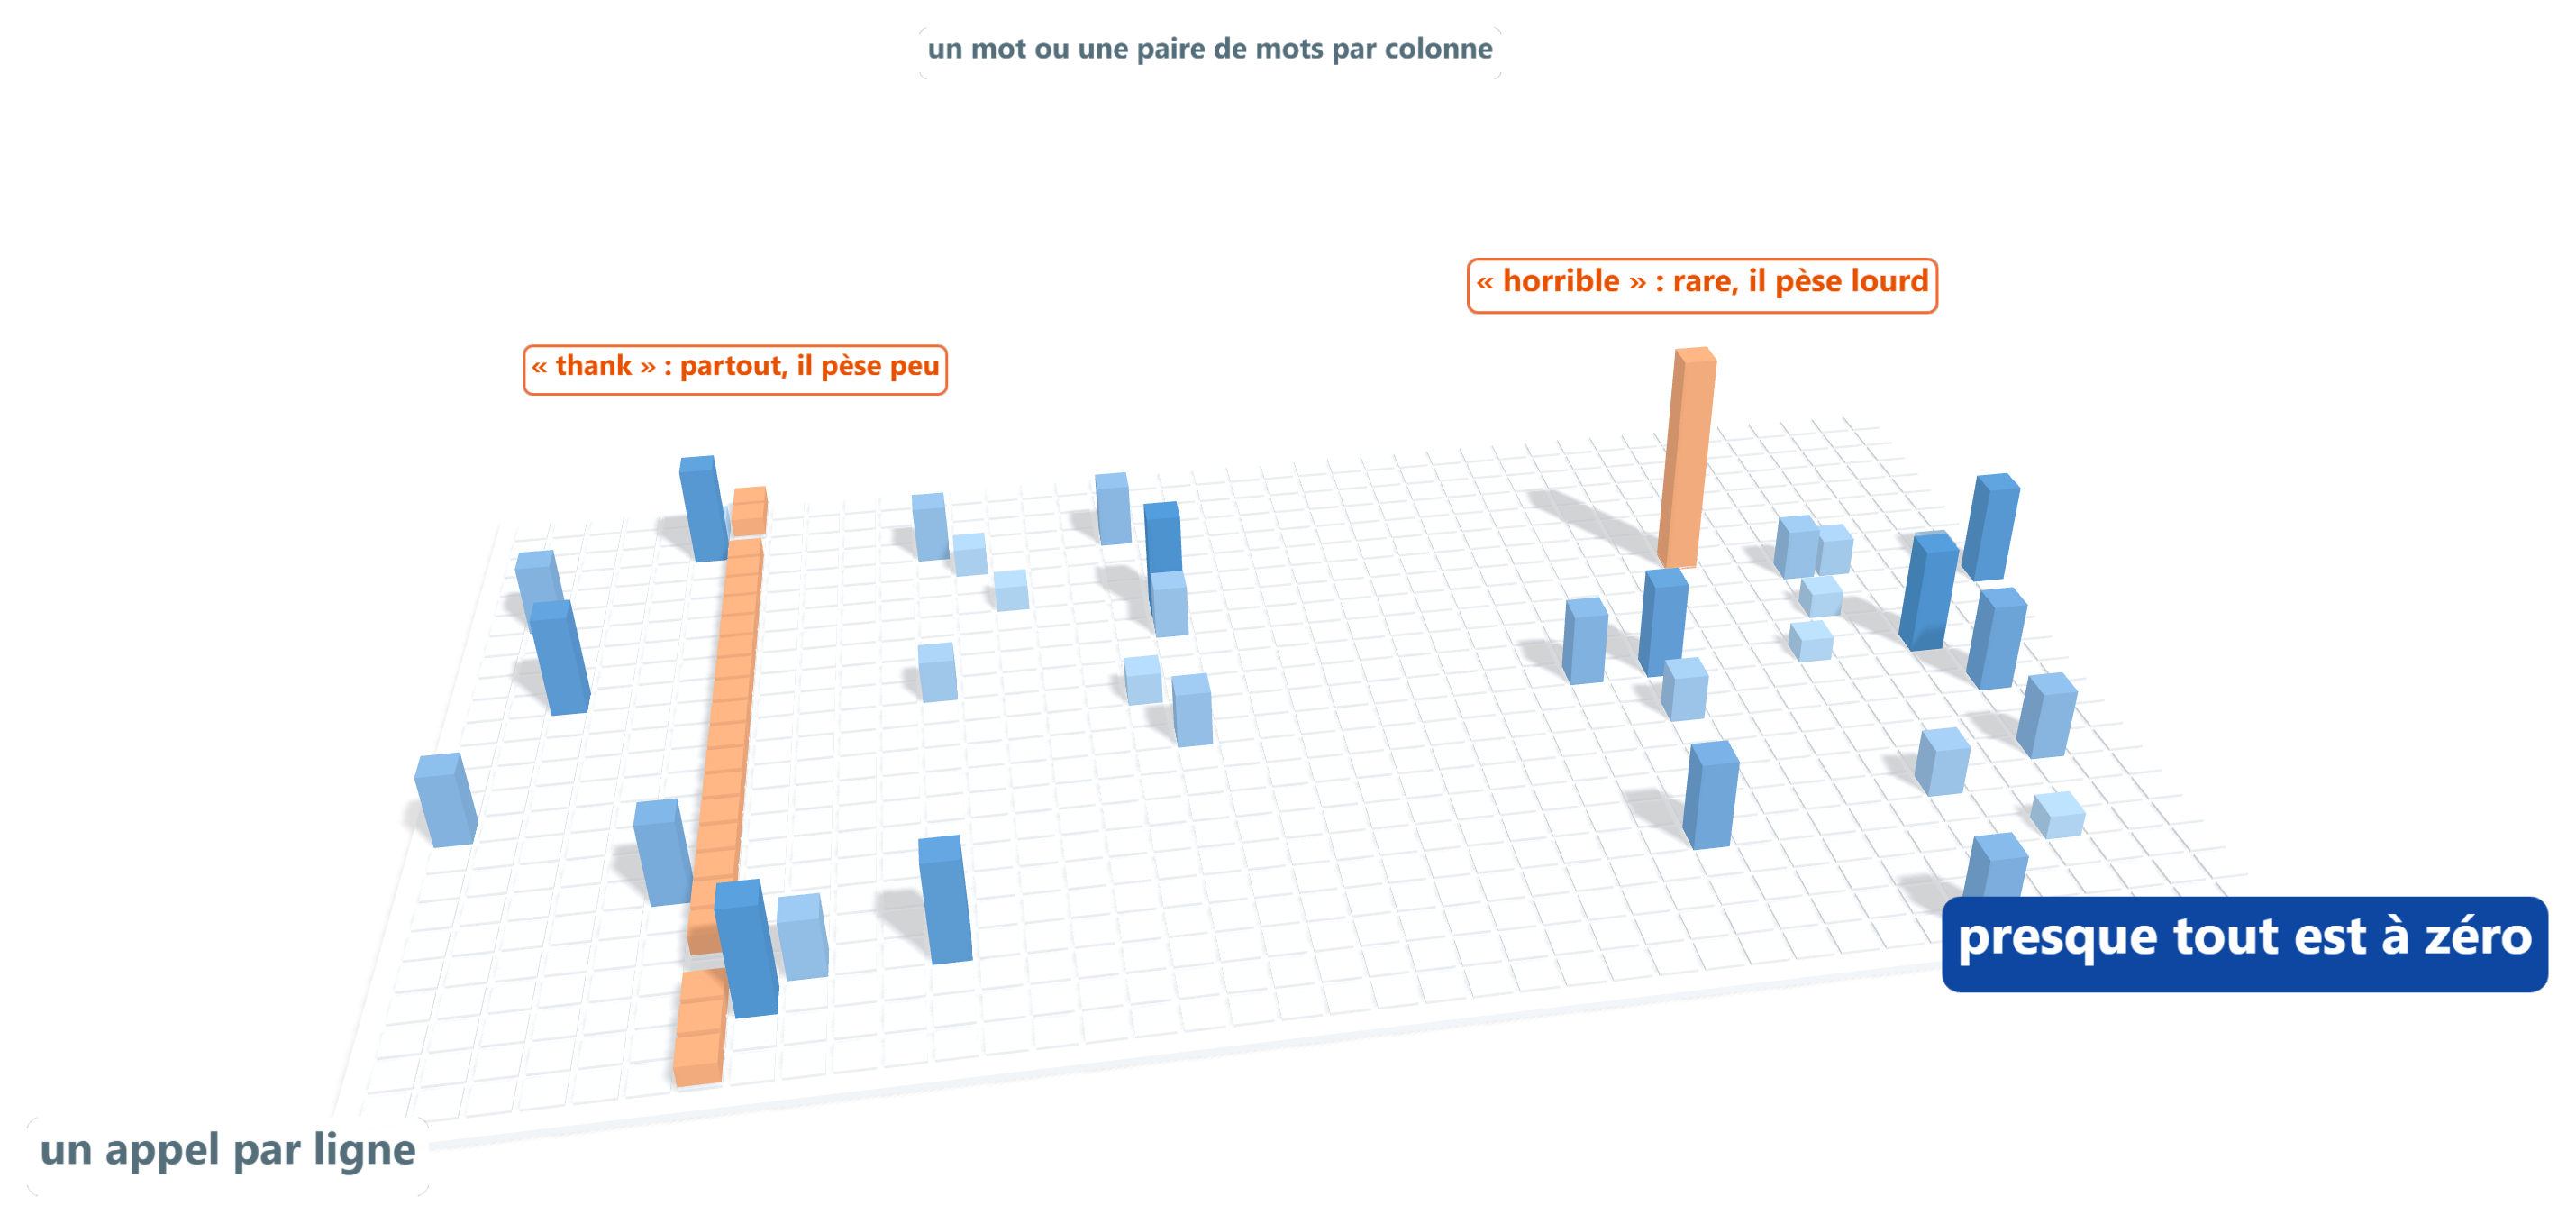
\includegraphics[width=0.8\linewidth]{3d_tfidf.png}
\end{center}

\begin{formulabox}
\centering\large TF-IDF $=$ \textbf{TF} {\small (le mot est-il \emph{ici} ?)} $\times$ \textbf{IDF} {\small (est-il \emph{rare} ailleurs ?)}
\end{formulabox}

\begin{center}
\begin{tikzpicture}[x=1.35cm, y=0.55cm]
\foreach \m/\n/\v [count=\i from 0] in {my/1\,422/1.02, thank/1\,040/1.33, bye/413/2.25, address/252/2.74, card/189/3.03, appreciate/8/6.08} {
  \pgfmathsetmacro{\c}{\v/6.08*100}
  \fill[sectioncolor!\c!skyblue] (0,-\i-0.35) rectangle (\v,-\i+0.35);
  \node[anchor=east, font=\small\ttfamily] at (-0.1,-\i) {\m};
  \node[anchor=west, font=\small] at (\v+0.08,-\i) {\textbf{\v} {\color{slate}\footnotesize dans \n{} appels}};
}
\node[font=\small\bfseries, color=darkblue] at (3,1.0) {IDF sur les 1\,446 appels du TP : plus rare = plus lourd};
\end{tikzpicture}
\end{center}

\begin{tcbraster}[raster columns=2, raster equal height, raster column skip=8pt]
\begin{enfant}[unbreakable]
\textbf{Un sac de mots} : on vide la phrase dans un sac et on compte, en donnant plus de poids aux mots
rares. Le sac sait que \og horrible \fg{} est dedans, pas qu'on a dit \og pas horrible \fg{}.
\end{enfant}
\begin{kpibox}[title={\faCalculator\ Dans ton TP}, unbreakable]
\small \textbf{2\,220} colonnes, \textbf{97,7\,\%} de zéros, \textbf{47} mots allumés par appel. Le
premier appel ressort avec \og debit card \fg{} : le TF-IDF a trouvé seul de quoi il parle.
\end{kpibox}
\end{tcbraster}

\begin{tcbraster}[raster columns=3, raster equal height, raster column skip=6pt]
\begin{kpibox}[title={\texttt{ngram\_range=(1, 2)}}, unbreakable]
\small mots seuls \textbf{et} paires de mots : \og thank \fg{} et \og thank you \fg{}
\end{kpibox}
\begin{kpibox}[title={\texttt{min\_df=2}}, unbreakable]
\small on jette les mots vus dans un seul appel
\end{kpibox}
\begin{kpibox}[title={\texttt{sublinear\_tf=True}}, unbreakable]
\small un mot répété dix fois ne compte pas dix fois plus
\end{kpibox}
\end{tcbraster}

\begin{stepbox}[title={4.3\quad Ton premier classifieur de texte}]
\begin{lstlisting}
def modele_texte():
    return make_pipeline(
        TfidfVectorizer(ngram_range=(1, 2), min_df=2, sublinear_tf=True),
        LogisticRegression(C=1.0, max_iter=3000, class_weight="balanced"))
\end{lstlisting}
\doisvoir{AUC proche de \textbf{0,86}, nettement au-dessus du repère \og motif seul \fg{} (0,637).}
\end{stepbox}

\begin{tcbraster}[raster columns=2, raster equal height, raster column skip=8pt]
\begin{kpibox}[title={\faBalanceScale\ \texttt{class\_weight="balanced"}}, unbreakable]
\small 25\,\% d'appels à 1, 75\,\% à 0 : sans ce réglage, le modèle répondrait \og 0 \fg{} partout.
\end{kpibox}
\begin{kpibox}[title={\faEye\ \texttt{mots\_marquants}}, unbreakable]
\small Les poids se lisent : un poids positif tire vers \og valence basse \fg{}, un poids négatif vers
\og valence haute \fg{}.
\end{kpibox}
\end{tcbraster}

\section{Deux questions qu'on te posera}

\begin{tcbraster}[raster columns=2, raster equal height, raster column skip=8pt]
\begin{kpibox}[title={\faQuestionCircle\ Logistique ou linéaire ?}, unbreakable]
\small \textbf{Linéaire} : un nombre quelconque, pour une quantité (une durée, une valence).\\
\textbf{Logistique} : un nombre entre 0 et 1, la probabilité d'une classe. Malgré son nom, c'est un
\textbf{classifieur}.
\end{kpibox}
\begin{kpibox}[title={\faQuestionCircle\ Pourquoi deux classes ?}, unbreakable]
\small La valence a une échelle arbitraire, la valeur est dans les extrêmes, et la décision est
binaire : on rappelle le client, ou non.
\image{Le thermomètre affiche 37,8 ; le médecin décide \og fièvre \fg{} ou \og pas fièvre \fg{}.}
\end{kpibox}
\end{tcbraster}

\section{Et trois ou cinq classes ?}

\begin{center}
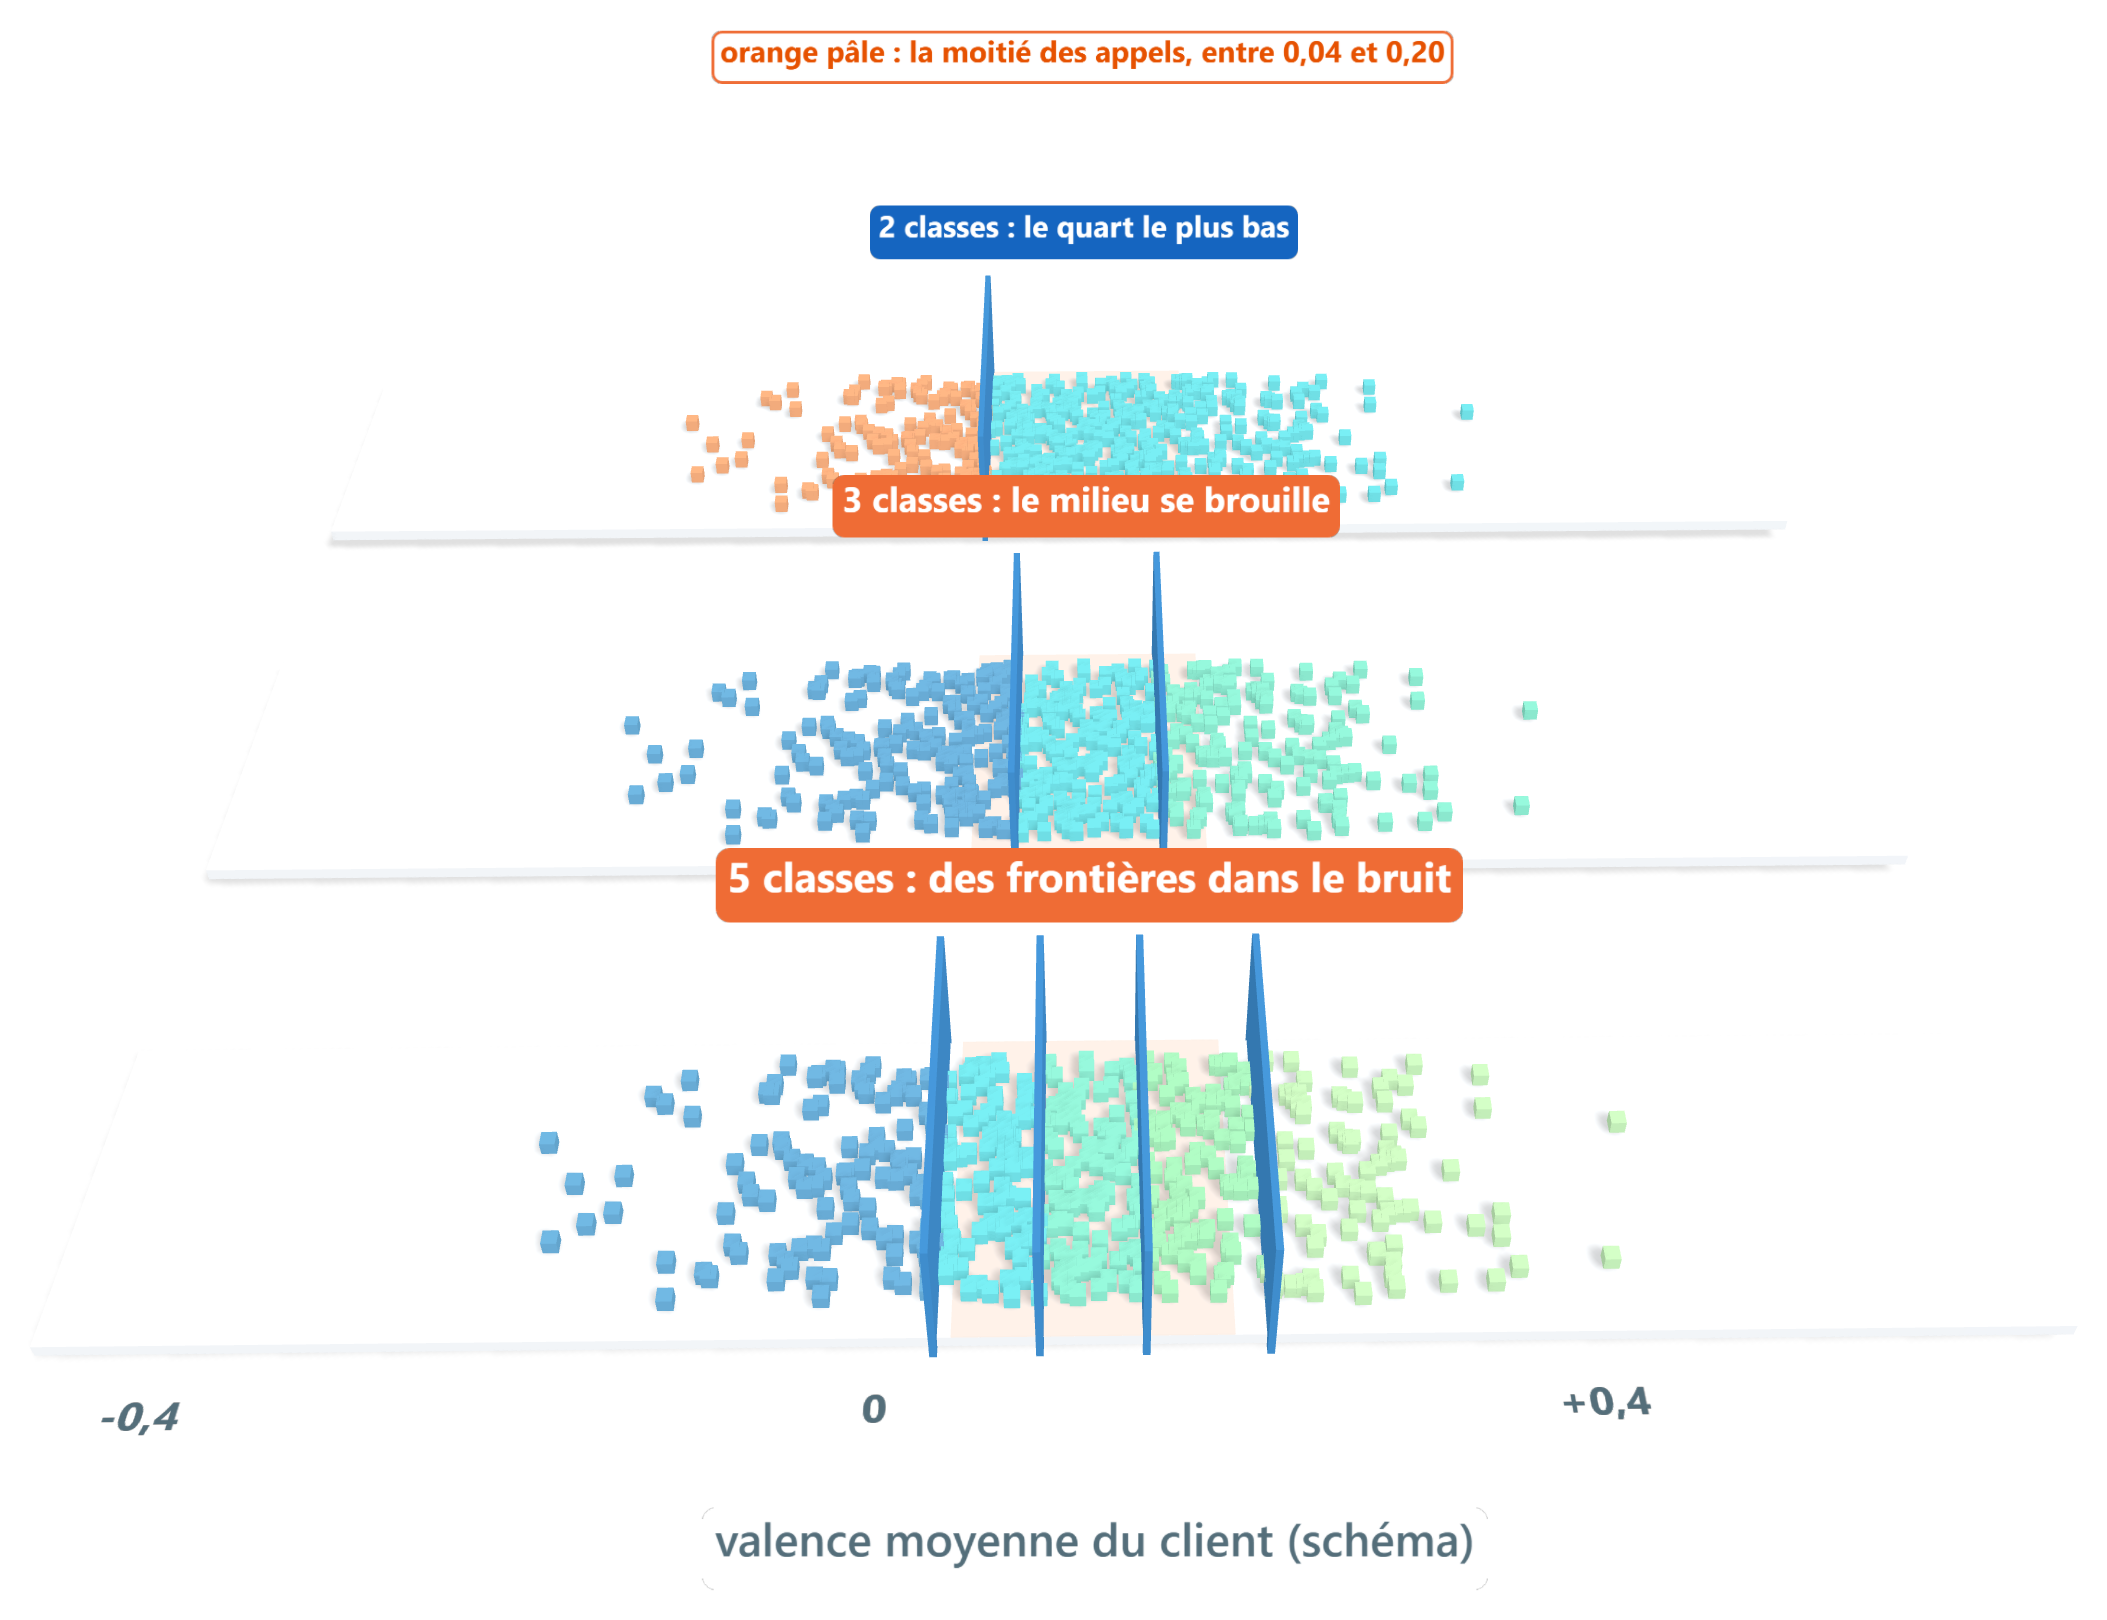
\includegraphics[width=0.72\linewidth]{3d_coupes.png}
\end{center}

\begin{tcbraster}[raster columns=3, raster equal height, raster column skip=6pt]
\begin{kpibox}[title={2 classes}, unbreakable]
\small AUC \textbf{0,849} : le quart le plus bas se reconnaît.
\end{kpibox}
\begin{kpibox}[title={3 classes}, colframe=orange!80!red, colbacktitle=orange!80!red, unbreakable]
\small extrêmes : AUC \textbf{0,85} ; milieu : \textbf{0,66}, presque au niveau du motif seul.
\end{kpibox}
\begin{kpibox}[title={5 classes}, colframe=orange!80!red, colbacktitle=orange!80!red, unbreakable]
\small 40\,\% de bonnes réponses ; \og plutôt bas \fg{} ou \og plutôt haut \fg{}, pas mieux.
\end{kpibox}
\end{tcbraster}

\begin{enfant}
\textbf{Ranger des enfants presque de la même taille en cinq rangs} : on repère les plus grands et les
plus petits, mais au milieu, c'est le hasard qui décide. Plus de rangs, ce n'est pas plus
d'information, ce sont plus de frontières arbitraires.
\end{enfant}

\section{La branche A bis : les modèles déjà entraînés}

\begin{center}
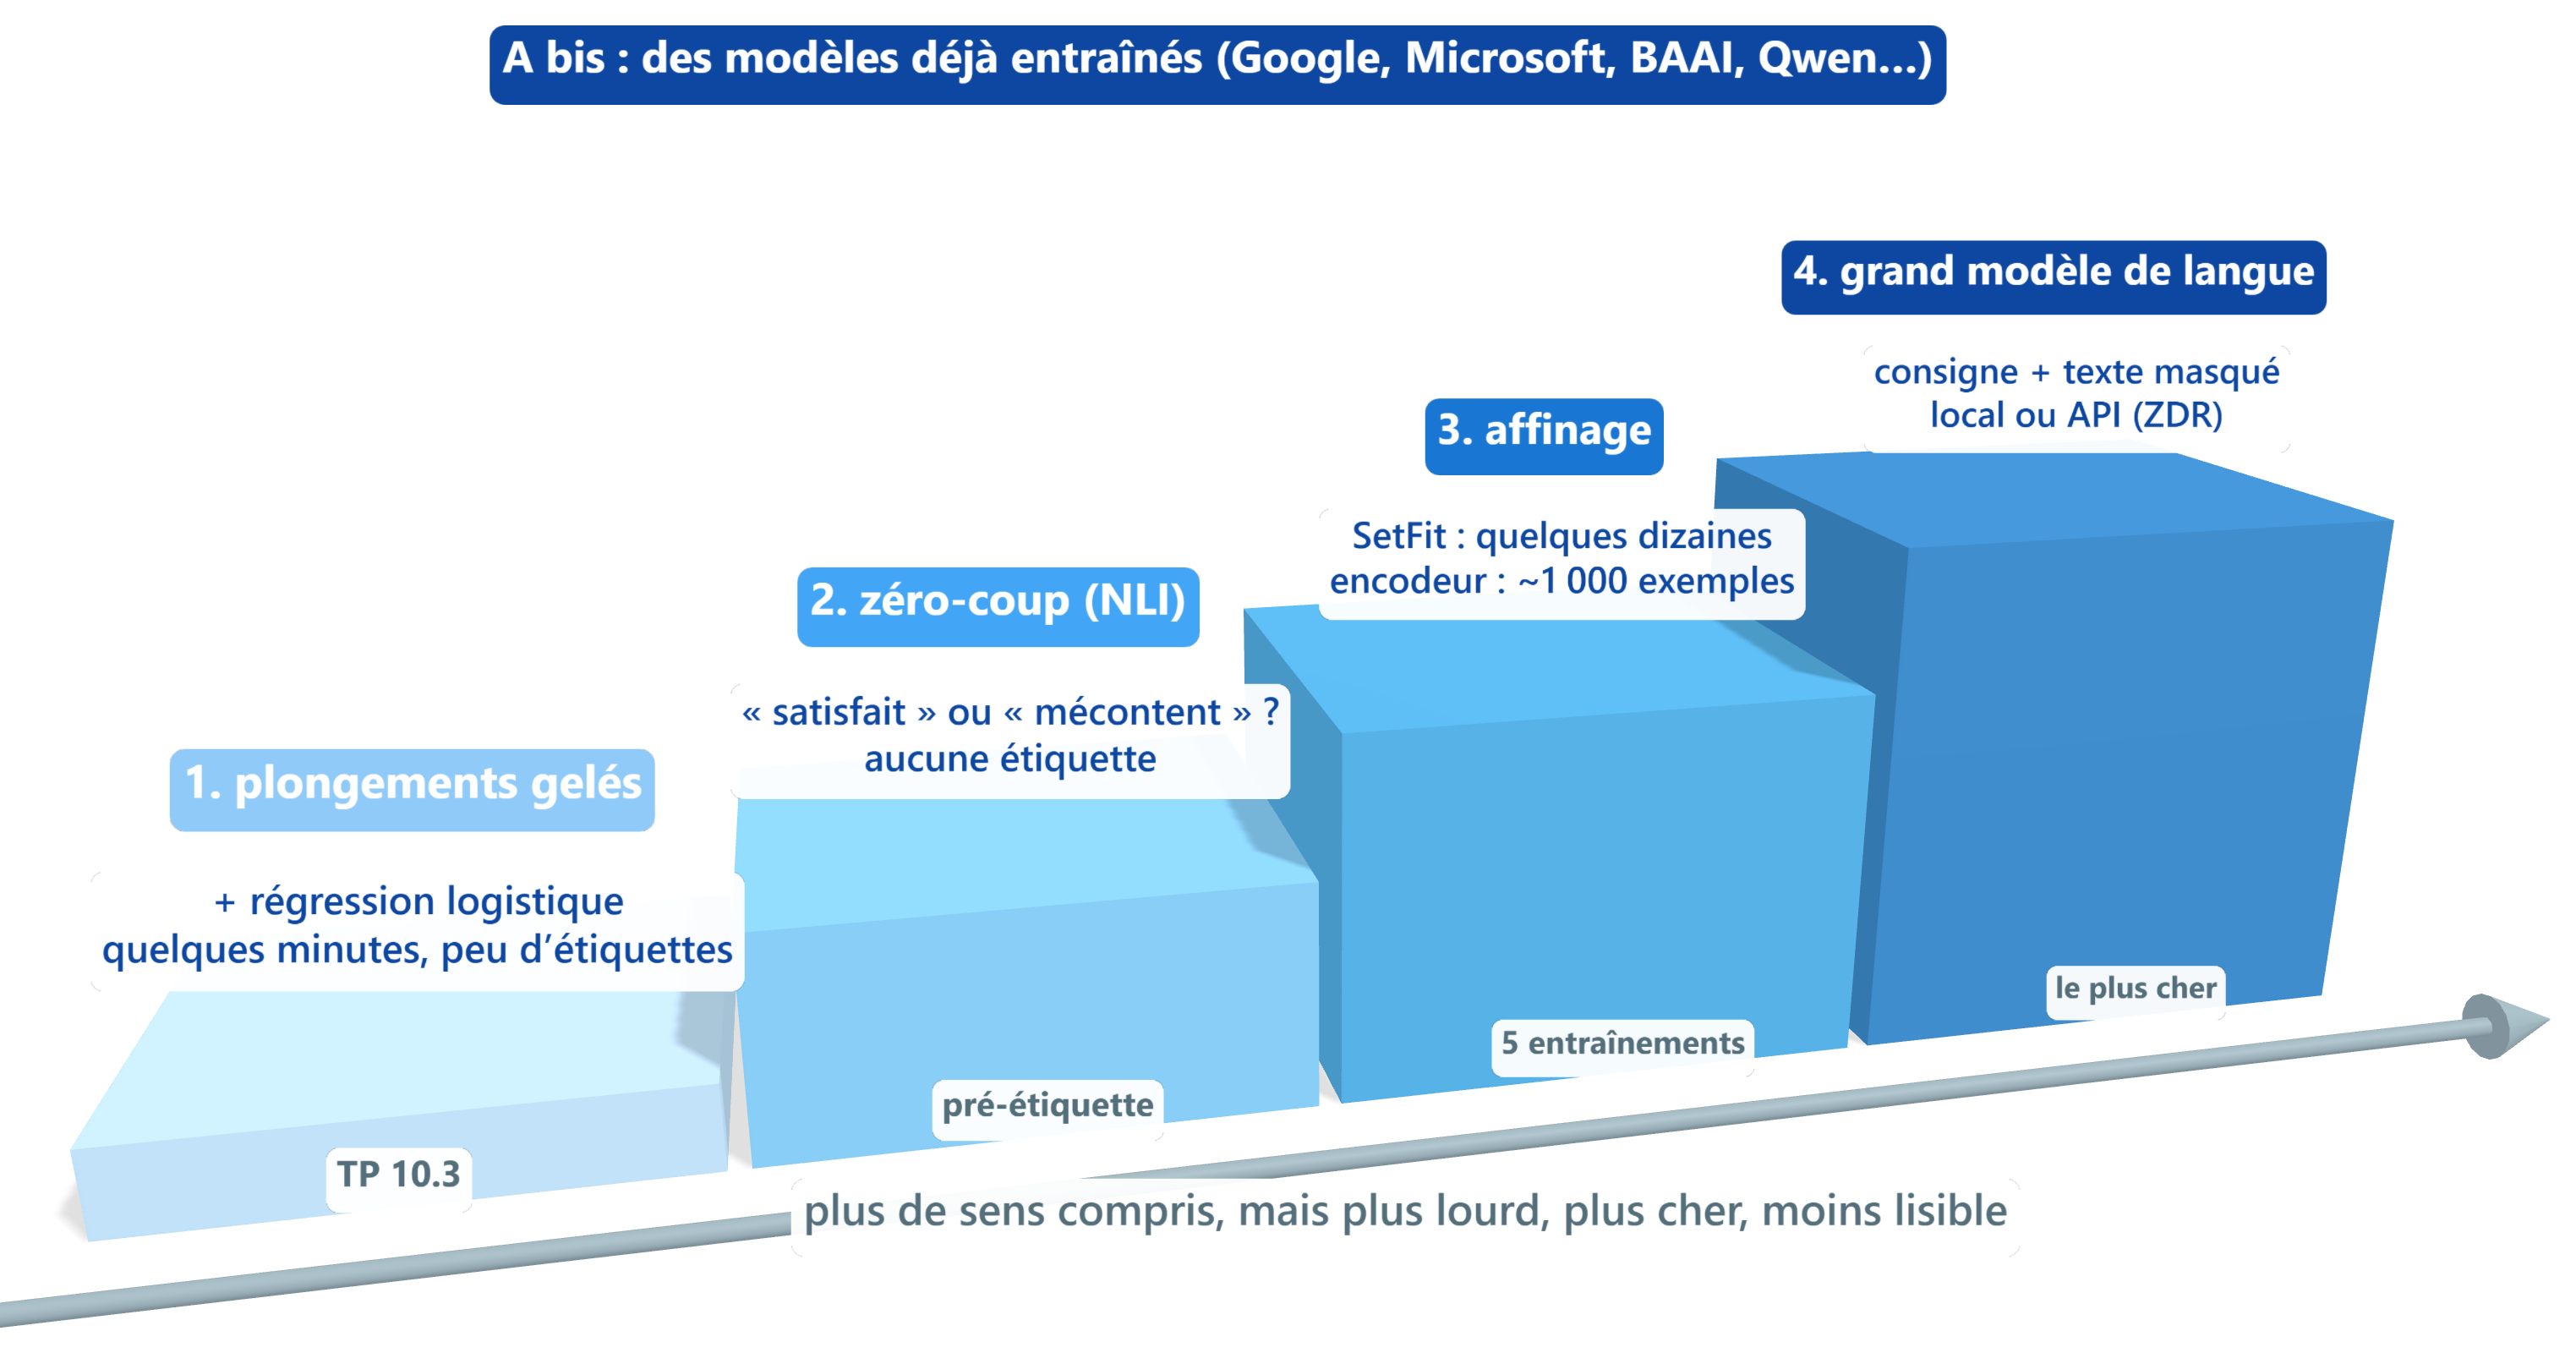
\includegraphics[width=0.85\linewidth]{3d_escalier.png}
\end{center}

\begin{tcbraster}[raster columns=2, raster equal height, raster column skip=8pt]
\begin{kpibox}[title={1. Plongements gelés (exercice 10.3)}, unbreakable]
\small un modèle de phrases donne un vecteur de \textbf{sens} par appel, puis la même régression
logistique. Pour le français : \texttt{intfloat/multilingual-e5-base}.
\end{kpibox}
\begin{kpibox}[title={2. Zéro-coup}, unbreakable]
\small \og satisfait \fg{} ou \og mécontent \fg{} ? sans aucune étiquette. Une \textbf{pré-étiquette},
pas une branche.
\end{kpibox}
\begin{kpibox}[title={3. Affinage}, unbreakable]
\small SetFit avec quelques dizaines d'exemples ; un encodeur complet avec un millier. \textbf{Un
entraînement par pli.}
\end{kpibox}
\begin{kpibox}[title={4. Grand modèle de langue}, unbreakable]
\small une consigne + le texte \textbf{masqué}. Le plus puissant, le plus cher ; il se juge comme un outil
de sentiment.
\end{kpibox}
\end{tcbraster}

\begin{stepbox}[title={\faPlug\quad La brancher}]
A bis donne \texttt{scores\_A2}, un score par appel, comme toutes les branches : fusion, ablation,
bootstrap, sans rien changer d'autre.\par\smallskip
\textbf{La seule question :} apporte-t-elle quelque chose que le TF-IDF n'a pas ?
\end{stepbox}

\begin{enfant}
\textbf{Le TF-IDF compte les mots ; un modèle pré-entraîné a déjà lu des milliards de phrases.} Il sait
que \og merci beaucoup \fg{} et \og c'est très gentil \fg{} veulent presque dire la même chose.
\end{enfant}

\subsection*{Le match : TF-IDF contre Google contre Qwen}

\begin{center}
\begin{tikzpicture}[
  r/.style={draw=#1, fill=#1!10, rounded corners=6pt, text width=3.3cm, align=center, font=\small,
    minimum height=1.2cm, inner sep=4pt},
  fl/.style={-{Stealth[length=2.5mm]}, thick, color=slate}]
\node[r=sectioncolor] (a) {\textbf{TF-IDF}\\(la branche A)};
\node[r=darkblue, below=0.25cm of a] (g) {\textbf{Google}\\{\scriptsize\texttt{embeddinggemma-300m}}};
\node[r=accentblue, below=0.25cm of g] (q) {\textbf{Qwen}\\{\scriptsize\texttt{Qwen3-Embedding-0.6B}}};
\node[draw=darkblue, fill=notebg, rounded corners=6pt, text width=3.0cm, align=center, font=\small, minimum height=4.2cm, right=1.0cm of g] (lr) {\textbf{même texte masqué}\\\textbf{même classifieur}\\\textbf{mêmes plis}};
\node[draw=orange!80!red, fill=orange!8, rounded corners=6pt, text width=3.6cm, align=center, font=\small, minimum height=4.2cm, right=1.0cm of lr] (v) {\textbf{verdict}\\[3pt]gain sur le TF-IDF, avec son intervalle\\[3pt]borne basse $> 0$ ?\\oui : on change\\non : on garde le TF-IDF};
\foreach \n in {a,g,q} \draw[fl] (\n) -- (lr.west |- \n);
\draw[fl, very thick] (lr) -- (v);
\end{tikzpicture}
\end{center}

\begin{piege}
\textbf{Ni \og le meilleur score \fg{}, ni \og la moyenne \fg{}.} Garder le meilleur des trois, c'est
garder le lancer de dé chanceux ; la moyenne donne le même poids au médiocre qu'au bon. On change
seulement si le gain est \textbf{net} (bootstrap apparié), et la \textbf{fusion apprise} pondère elle-même
les représentations ; elle n'est gardée que si elle bat nettement la meilleure seule.
\end{piege}

\begin{piege}
\textbf{Pourquoi pas tout de suite un réseau de neurones ?} Avec 1\,446 appels, ce modèle simple est
difficile à battre, il s'entraîne en une seconde, et ses poids se lisent. On ne sait si un modèle plus
gros apporte quelque chose qu'en le comparant à celui-ci.
\end{piege}
